\documentclass[a4paper,12pt]{article}
\usepackage[utf8]{inputenc}
\usepackage[T1]{fontenc}
\usepackage[spanish]{babel}
\usepackage{csquotes}
\usepackage{anysize}
\usepackage{graphicx}
\marginsize{25mm}{25mm}{25mm}{25mm}

\title{Foraging in a simulated environment: There's a rat loose in the lab}
\author{Roger L. Mellgren}
\date{1982}

\begin{document}
{\scshape\bfseries \maketitle}

Los psicólogos se están volviendo menos miopes y están ampliando sus marcos de referencia teóricos. Toman en cuenta modelos económicos, ecología, y etología. Hay nueva apreciación por la ``naturaleza'' de la conducta, por lo que se ha buscado usar situaciones de aprendizaje que requieran que los animales pasen un tiempo significativo en la situación y que trabajen para obtener la totalidad de su comida/agua en ese tiempo.

Este experimento busca desarrollar un procedimiento más natural, pero manteniendo control experimental. Para ello se permite a las rata forrajear por su comida en un cuarto que contiene parches de comida compuestos por cajas que contienen arena con comida enterrada. La habitación estaba ordenada caprichosamente. Se conocía el contenido de cada parche y solo un sujeto forrajeaba a la vez, con lo que es posible hacer una prueba cuantitativa de la teoría de forrajeo óptimo. La teoría indica que un depredador capturará presas en un parche para maximizar la tasa de ganancias relativa al ambiente completo.

La conducta de forrajeo óptimo en este experimento es una función de la cantidad de comida disponible en cada parche. Se asume (1) que el tiempo entre capturas sucesivas está inversamente relacionado con el número de presas disponibles en el parche (es decir, se encuentra más rápido una presa cuando éstas son más abundantes), (2) el costo de buscar una presa en un parche es relativamente mayor que el costo de viajar de un parche a otro (de no ser costoso, el depredador simplemente agotaría un parche antes de pasar al siguiente). Así, un depredador óptimo minimizará el tiempo pasado buscando dentro de un parche dado que es el costo principal de la función. 

La forma de la solución óptima para la depredación en un ambiente distribuido en parches depende de la naturaleza del ambiente y las restricciones del depredador. Por ejemplo, si se imponen restricciones en el viaje (como barreras físicas o peligros) la estrategia óptima sería agotar un parche en un grado mayor.

En este experimento había 9 parches disponibles con distintos números de presas. Se asume que el costo de viajar es menor que el de buscar dentro de un parche. La estrategia óptima sería explotar cada parche hasta un cierto nivel determinado por la cantidad total de comida a recolectar y la distribución de comida entre los parches. La cantidad de comida se varió en incrementos de 3 y 5 pellets por parche, con lo que la estrategia óptima se puede expresar como una relación lineal entre el número disponible y la cantidad comida. Esta predicción es consistente con la idea de que el depredador tiene un tiempo de corte para capturas sucesivas de presas, y que una vez se llega a este tiempo de corte sin encontrar a una presa, el depredador ``se rinde'' y pasa a otro parche.

{\scshape\bfseries Method}

Se utilizó una habitación grande sin ventanas y varias habitaciones menores. Los parches eran cajas llenas de arena con una profundidad de aproximadamente 4cm. La habitación se mantenía casi en oscuridad. La comida eran pellets firmes, y se proveyó además agua en dos botellas dentro de la habitación.

Las ratas tuvieron experiencia extensiva forrajeando por comida enterrada en arena antes de comenzar el experimento.

{\itshape Fase 1.} Había 15 pellets disponibles por parche en las primeras 5 sesiones y 20 en las últimas 4. Las sesiones eran de 12 horas. A las 9 am y 9 pm se cambiaba la rata, se hacían mediciones y se reiniciaba la habitación.

{\itshape Fase 2.} Duró 6 sesiones. Los parches tuvieron números distintos de pellets según la figura 1. Las sesiones aún duraban 12 horas. 

\begin{figure}[hb]
	\begin{center}
		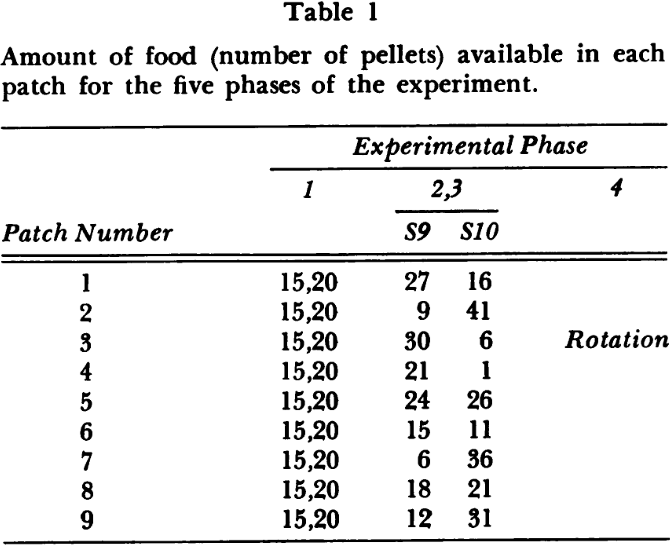
\includegraphics[scale=0.5]{Mellgren1982(1).png}
	\end{center}	
\end{figure}

{\itshape Fase 3.} Duró 15 sesiones. Fue idéntica a la fase 2 salvo porque las sesiones duraron solo 1 hora.

{\itshape Fase 4.} Duró 9 sesiones de 1 hora. El número de pellets fue rotado de modo que cada número de pellets fuese encontrado una vez en cada parche. 

La arena era mezclada y redistribuida constantemente para evitar efectos del olor. Solo se proporcionó comida adicional durante las fases 3 y 4 para mantener el peso al 80\%.

Se registró el número de pellets comidos, las heces, la orina, el agua consumida y el peso de la rata al comienzo y al final de la sesión. También se registró la ubicación de la rata en el momento en que el experimentador entró en la habitación al final de la sesión.

{\scshape\bfseries Results and discussion}

Se verán los datos primero de forma neutral y después con relación a la teoría de optimalidad.

{\scshape Descriptive account}

Los sujetos aprendieron rápidamente la localización de todos los parches. Aunque en ocasiones no se tomó comida de algún parche, casi siempre se encontró alguna indicación de que fue, cuando menos, visitado y que ocurrió alguna forma de forrajeo.

Las heces se encontraron casi siempre en los parches. Ambas ratas adoptaron una casa en una de las esquinas de la habitación. En las primeras fases las ratas eran frecuentemente encontradas ahí al terminar las sesiones. En las últimas, con menos tiempo disponible, eran encontradas en campo más abierto, pero corrían rápidamente a la casa.

Se usaron coeficientes de correlación para indicar el grado de la relación entre las densidades de los parches y su utilización.  Se correlacionó la cantidad total de comida disponible en un parche con la cantidad consumida en el mismo. En un principio la correlación fue de -.41 para una rata (lo que indica que comía más en los parches menos densos) y de .66 para la otra. Hacia el final las correlaciones fueron de .35 y .71, lo que indica que ajustaron su forrajeo para adecuarse a la distribución de la comida.

En la fase 4 la densidad de comida fue movida entre los parches. Se computaron nuevas correlaciones. En este caso una correlación alta indicaría que un sujeto fue sensible a la densidad del parche, y una baja que fue principalmente sensible a la localización. Las correlaciones en este caso fueron de .85 y .18.

Ambos hallazgos indican que la primera rata se vio forzada a ajustar sus patrones de forrajeo para sobreponerse a una preferencia por la posición que ya tenía, y la forma de hacerlo fue incrementando su sensibilidad a la densidad de los parches. La otra rata enfrentó poca presión para hacer lo mismo dado que sus preferencias ya eran consistentes con la distribución de la comida, así que no fue igualmente sensible a la densidad.

Se consumió muy poca agua durante las sesiones, regularmente menos de 10ml. 

{\scshape Optimal foraging theory}

Según esta teoría, los animales actuarán para optimizar sus patrones de forrajeo y maximizar las ganancias. 

Las pruebas usuales de la teoría manipulan una sola variable a la vez (tamaño de la presa, tiempo de viaje). Este experimento buscaba igualmente manipular una sola variable: la densidad de presas.

Las predicciones de la teoría fueron derivadas tomando el número total de pellets consumidos por cada animal y determinando el patrón óptimo de utilización de parches bajo los supuestos de que (1) los costos de búsqueda incrementan según disminuye la disponibilidad de la presas, y (2) hay un costo mayor por buscar dentro de un mismo parche que por viajar a otro. El ajuste de los datos con la teoría no es impresionante.

Las desviaciones de las predicciones son sistemáticas: los parches con bajas densidades de presas son sobre-utilizados, y aquellos con altas densidades son bajo-utilizados. Esto indica que, según la teoría, los sujetos son conservadores. No explotan los parches en el grado en que se esperaría, y en lugar de ello muestrean de parches de menor densidad, sobre-explotándolos. 

Aun si se cambian los supuestos y se asume que el tiempo de viaje es más costoso, el ajuste sigue sin ser bueno (de hecho empeora). Esto es similar al patrón mostrado por los humanos, que bajo-utilizan el valor diagnóstico de la información con respecto a lo óptimo,  tomando una aproximación más conservadora.

La teoría de forrajeo óptimo hace predicciones idénticas sobre el uso de parches sin importar que las densidades mantengan localizaciones constantes o se varíen en forma no sistemática. La única diferencia es que cuando las densidades varían en localización, le llevará tiempo a los sujetos descubrir la distribución, por lo que será más probable que los parches pobres se sobre-exploten.

En la fase 4 del experimento la segunda rata mostró las mismas desviaciones con respecto a la teoría de forrajeo óptimo. En cambio, la primera rata no se desvió significativamente de las predicciones de la teoría (si se excluyen los dos parches de menor densidad). Esto de nuevo apoya la idea de que la primera rata fue forzada a ser más sensible a las densidades dada la disparidad entre sus preferencias iniciales y la distribución real. Parece ser que el forrajeo óptimo no es un resultado necesario de la programación biológica, sino que depende de la forma en que ésta interactúa con el ambiente.

Los resultados principales son:
\begin{enumerate}
	\item Las ratas son muestreadoras exhaustivas de sus fuentes de comida.
	\item Las ratas tienden a ser conservadoras en el sentido de que prefieren una localización de forrajeo por encima de aquello que está realmente disponible en ella, salvo cuando las localizaciones preferidas tienen cantidades muy pequeñas de comida.
	\item Si hay una disparidad entre las localizaciones preferidas y la riqueza del ambiente, se incrementa la sensibilidad a ésta riqueza.
\end{enumerate}

Es interesante que un sujeto mostró conducta más eficiente en un ambiente cambiante que en uno estable. Esto puede indicar que hay distintos tipos de aprendizaje involucrados en tareas así de complejas: aprender dónde están las fuentes de comida y aprender sobre su naturaleza y cómo obtener la comida.

En conclusión, el procedimiento descrito es un método efectivo para evaluar la operación de variables que afectan la conducta en el laboratorio y su interacción en una situación compleja.

\end{document}
